\section{El procés de recerca genealògica}

    \paragraph{}
    A tota persona que li interessi realitzar recerca genealògica sobre la seva pròpia família o la d'una persona propera, se li suggereix el següent procés com a mètode de treball\footfullcite{wiki:fsResearchProcess}.

    El procés de recerca es desenvolupa en cicles i cada cicle consta de cinc fases. A continuació, es detallen una a una:

    \begin{enumerate}
        \item \textbf{Identificar la informció coneguda:} Identificar i revisar tota la informació inicial que es coneix. Pel final de la fase s’haurien de tenir recopilats, ordenats i documentats, tots els esdevenimentals relacionats amb la família o persona a estudiar disponibles.
        \item \textbf{Decidir què es vol aprendre:} L’objectiu d’aquesta fase és identificar sobre quin individu es vol obtenir informació, què es vol aprendre d’aquesta persona i si és possible, el temps i lloc aproximat en què aquesta persona va viure.
        \item \textbf{Seleccionar els arxius a consultar:} Aquesta fase resulta la més complexa de tot el procés. L’objectiu, ordenar de més a menys útils les diferents fonts de dades a consultar i quins arxius resulten més interessants.
        \item \textbf{Obtenir i consultar els arxius:} Durant aquesta fase es consultaran les fonts de dades seleccionades a l’apartat anterior. Al final d’aquesta, hauríem de tenir anotat tot allò que s’ha descobert i còpies dels documents que suporten els descobriments, ja sigui en format de fotocòpies, notes o qualsevol altra mena de suport físic o digital.
        \item \textbf{Utilitzar la informació:} Finalment, en aquesta fase, tocarà avaluar la informació descoberta, transportar la nova informació als formularis adients, or\-ga\-nit\-zar la informació i compartir els resultats. Un cop finalitzades totes aquestes tasques, s'estarà preparat per tornar a iniciar la roda del procés i seguir així amb la recerca genealògica.
    \end{enumerate}

    \paragraph{}
    La figura~\ref{fig:researchProcess} mostra les cinc fases d'aquest procés cíclic.

    \begin{figure}[h]
            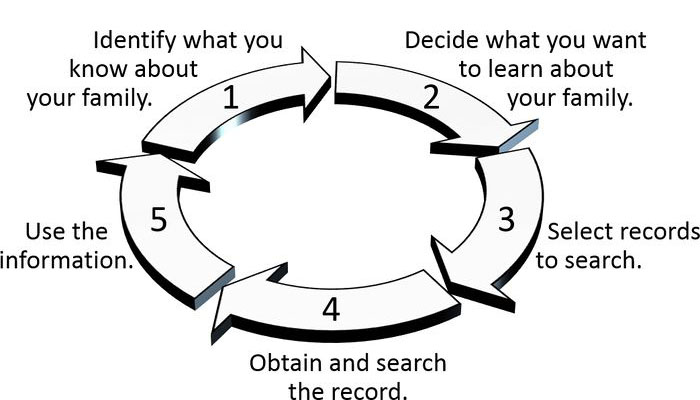
\includegraphics[scale=0.6]{02/researchProcess}
            \centering
            \caption{Procés de recerca genealògica.\label{fig:researchProcess}}
    \end{figure}
